\section{Hidden comunication by targeted reflections}

\subsection{RIS Diagonalization}

We will start from the paper \textit{Reconfigurable Intelligent Surface: Reflection Design Against Passive Eavesdropping} \cite{9328149}, explaining how to hide communication between two actors from eavesdroppers using Reconfigurable Intelligent Surfaces, then expanding it to multiple receiving users at the same time.

\begin{figure}[H]
  \centering
  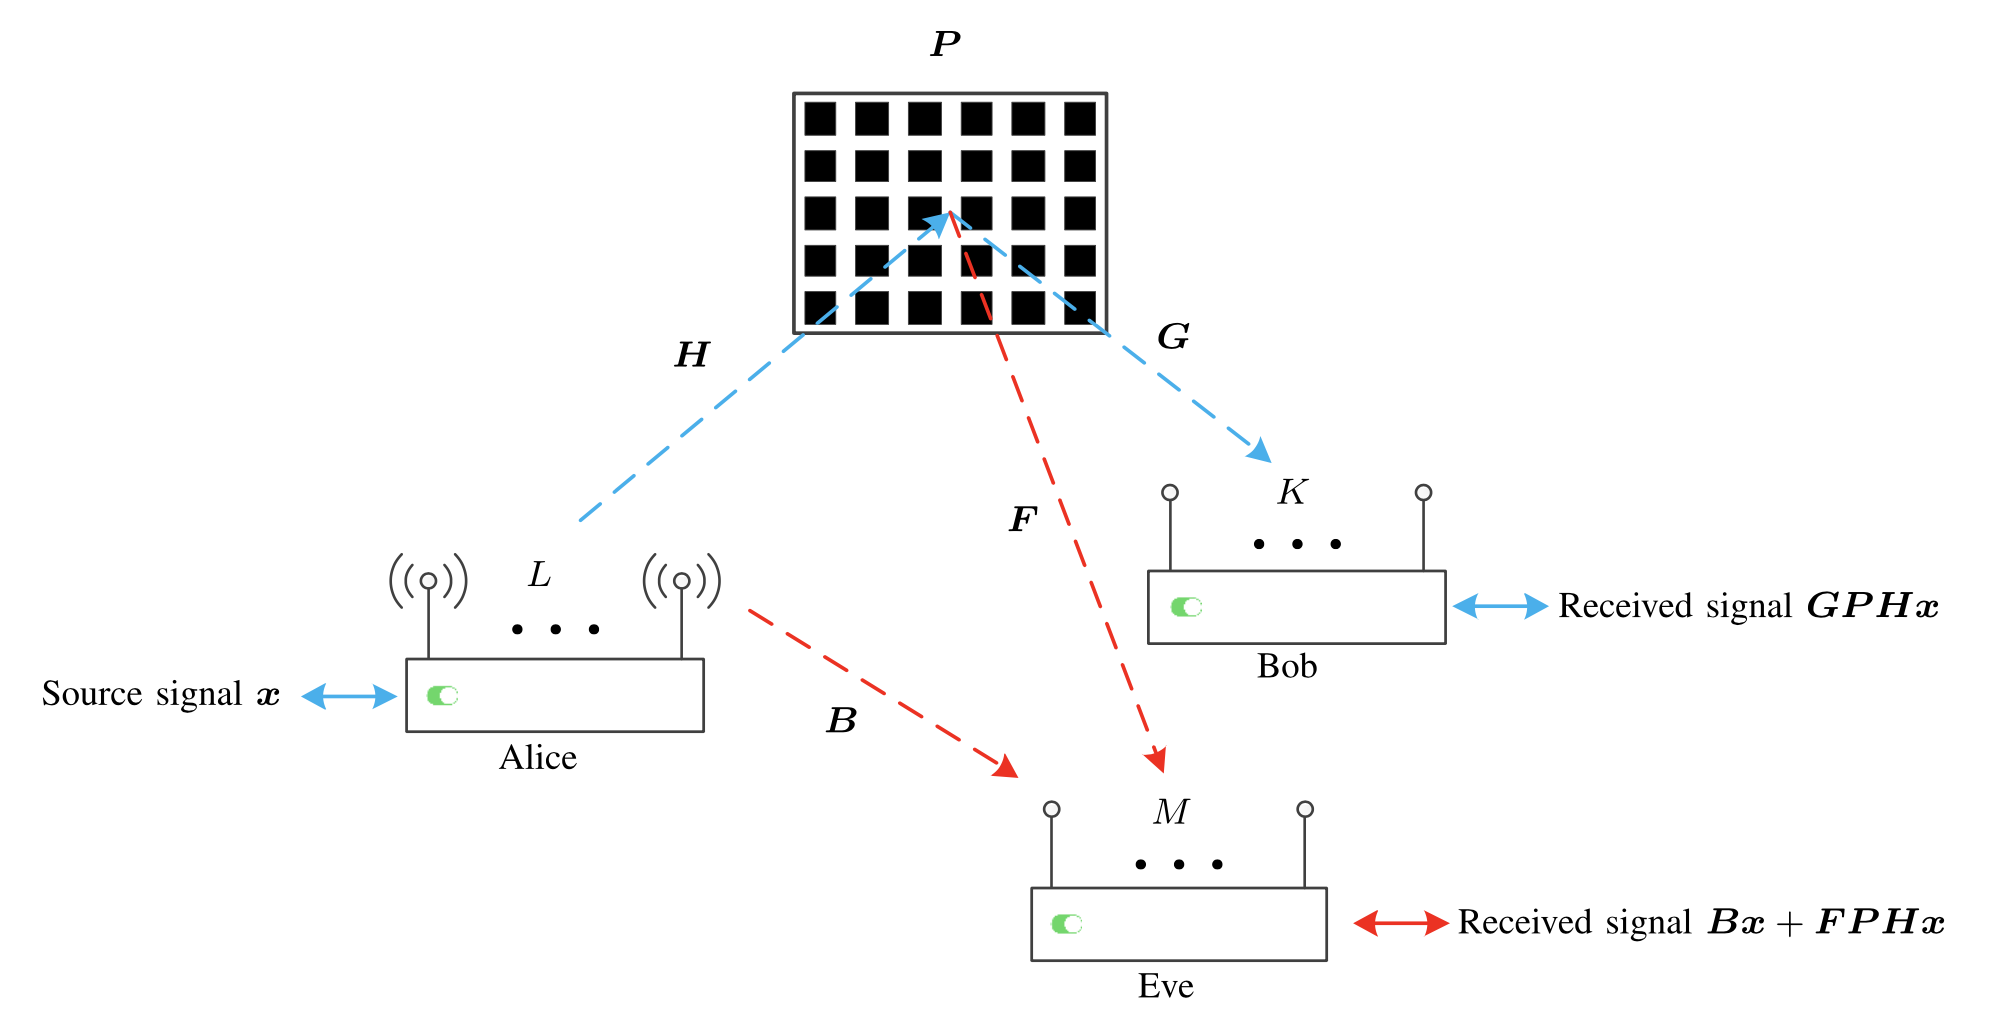
\includegraphics[width=\linewidth]{imgs/problem-description.png}
  \caption{Setup of the system [From \cite{9328149}]}
  \label{fig:correlation_sk}
\end{figure}

In \cite{9328149}, the authors studied how to use RISs to allow communications between two users without LOS, while making the signal undeciphrable for eavesdroppers. We call $L$ the transmitter's antennas, $K$ the receiver's antennas, $M$ the eavesdropper's antenna, and $N$ the RIS reflecting elements. We assume $L \ge K \ge 2$.

We define $\bm{H} \in \C^{NxL}$ the channel response \footnote{A channel response for a MIMO communication is a matrix made of complex number, where the position $i,j$ indicates the signal received from antenna $j$ to antenna $i$} from the transmitter to the RIS, $\bm{G} \in \C^{KxN}$ the channel response from the RIS to the receiver, $\bm{P} = diag\{p\} \in \C^{NxN}$ a diagonal matrix in which the $n$th diagonal element represents the reflection coefficient of the $n$th unit at the RIS.

The objective is making the receiver's final signal $\bm{GPH}$ a diagonal matrix, while making every possible eavesdropper's final signal a full matrix.

We will leave for later the technical details of why this would achieve secrecy for the legitimate users or how the actors communicate with each others, and will just focus on the mathematics behind the calculation. It is possible to read more in the paper \textit{Space shift keying modulation for MIMO channels} \cite{5165332}, which we will summarize in a later chapter.

Our contribution to the field will be to generalize these calculations to $J$ receving users and $M$ RISs used in parallel and in sequence.

Formally, the condition we want to satisfy is:

\begin{equation}
  || [\bm{GPH}]_{:,1:K} - [[\bm{GPH}]_{:,1:K}]_{diag} || ^2 = 0
  \label{eq:diag_condition}
\end{equation}

Where $[GPH]_{:,1:K} \in \C^{KxK}$ denotes the first K columns of the matrix $\bm{GPH} \in \C^{KxL}$.

Given

\begin{equation}
  \bm{W} = \sum_{i,j = 1, i \ne j}^{K} (g_{j,:} \odot h_i^T)^H (g_{j,:} \odot h_i^T)
\end{equation}
\begin{equation}
  \rank(\bm{W}) = K(K-1)
\end{equation}
\begin{equation}
  \rank(\bm{W}) - \nullop(\bm{W}) = N
\end{equation}
Where $\nullop$ refers to the dimension of the $\nullop$ space.
\begin{equation}
  \nullop(\bm{W}) = N - (K^2 - K)
\end{equation}

The formula \eqref{eq:diag_condition} can be rewritten as

\begin{equation}Wp = 0\end{equation}

and the solutions of $p$ can be found in the $\nullop$ space of $\bm{W}$. Using singular value decomposition (SVD), we can decompose

\begin{equation}
  \bm{W} = \bm{R \Sigma V}^H
\end{equation}

With SVD, we have $\bm{\Sigma} = diag(\sigma) \in C^{NxN}$ a diagonal matrix. the first $\rank(\bm{W}) = K^2-K$ elements of $\sigma$ are non-zero, while the last $\nullop(\bm{W}) = N - (K^2-K)$ elements are zero \cite{svd}.

Given a more generic $\bm{A} \in \C^{mxn} = \bm{R}'\bm{ \Sigma}' \bm{V}'^H$, we have the column vectors of $R'$ being an orthonormal span of $C^m$, and the row vectors of $V'$ being an orthonormal span of $C^n$.

Suppose $\bm{A}$ is an Hermitian matrix (meaning $\bm{A} = \bm{A}^H$). This will be useful later, as $\bm{W}$ is also an Hermitian matrix by construction. Let's call $k$ the $\nullop$ space dimension of $\bm{A}$, and ,by the property above, the $\nullop$ space dimension of $\bm{A}^H$ too.

The last $k$ columns of $\bm{R}'$ are a span of the $\nullop$ space
\begin{equation}
  N(\bm{A}^H) = [r_{m-k}, ..., r_m ] \in \C^{mxk}
  \label{null-space-hermitian}
\end{equation}
while the last $k$ rows of $V'^H$ are a span of the $\nullop$ space
\begin{equation}
  N(\bm{A}) = \begin{bmatrix} v'^H_{n-k} \\ ... \\ v'^H_n \end{bmatrix} \in \C^{kxn}
  \label{null-space-normal}
\end{equation}
Being $\bm{A}$ an Hermitian matrix, the two $\nullop$ spaces are both solutions to $\bm{A}x = 0$.

Consider now $\bm{W} \in C^{NxN}$. The paper in question uses equation \eqref{null-space-hermitian} to find the solutions, since $W$ is hermitian and square. Taken $\bm{U} \in \C ^ {Nx(N-(K^2 - K))}$ the last $N-(K^2 - K)$ columns of the left singular matrix $\bm{R}$. $\bm{U} \in \bm{N}(\bm{W})$ for the explanation above. We then have

\begin{equation}\bm{WU} = 0\end{equation}
\begin{equation}p = \bm{U}q\end{equation}
\begin{equation}
  \bm{WU}q = 0
  \label{q_random_vector}
\end{equation}

being true, and $q \in \C^{N-(K^2 - K)}$ can be a random vector.
